\documentclass[11pt,a4paper]{article}
%\usepackage{natbib}
\usepackage[natbib=true, style=authoryear]{biblatex}
\addbibresource{citations.bib}
\usepackage[french]{babel}
\usepackage{textcomp}
\usepackage{csquotes}
\usepackage{setspace}
\usepackage{fancybox}
\usepackage{fancyhdr}
\setlength {\marginparwidth }{2cm}
\usepackage{todonotes}
\usepackage{lipsum}
\usepackage{amsmath}
\usepackage{amsfonts}
\usepackage{amssymb}
\usepackage{pifont}% http://ctan.org/pkg/pifont
\newcommand{\cmark}{\ding{51}}%
\newcommand{\xmark}{\ding{55}}%
\usepackage{bookmark}
\usepackage{mathtools}
\usepackage{scalerel}

\usepackage{diagbox, eqparbox, hhline}
% https://tex.stackexchange.com/questions/150634/how-to-force-a-text-to-appear-after-a-table
\usepackage{placeins}
\usepackage{graphicx}
\usepackage{booktabs}
\usepackage{lscape}
\graphicspath{{Img/}}
\usepackage{float}
\usepackage{titlesec}%remove chapter N
\usepackage{soul} % Texte surligné
\usepackage[left=2cm,right=2cm,top=2cm,bottom=3cm]{geometry}
\setlength{\parindent}{0cm}
\usepackage[framemethod=tikz]{mdframed} %highlight an entire paragraph
\usepackage{framed}
\usepackage{adjustbox}
\usepackage{array}
\usepackage{glossaries}


\usepackage{caption}



\usepackage{comment}


\usepackage{color,soul}
\usepackage{marginnote}
\hypersetup{
    colorlinks,
    citecolor=black,
    filecolor=black,
    linkcolor=black,
    urlcolor=blue
}

\usepackage{listings}
\lstset{
    numbers=left,
    numberstyle=\sffamily\tiny,
    escapeinside={<@}{@>}
}

\usepackage{pdfpages}

\usepackage{hyperref}

\setcounter{secnumdepth}{3}
\setcounter{tocdepth}{3}

\makeatother



\let\labelitemi\labelitemii



\setlength{\doublerulesep}{2.5pt}
\frenchbsetup{ItemLabeli=\textbullet}

\begin{document}
\newcommand{\JMUTitle}[9]{
    \thispagestyle{empty}
    \vspace*{\stretch{1}}
    {\parindent0cm
        \rule{\linewidth}{.7ex}}
    \begin{flushright}
        \vspace*{\stretch{1}}
        \bfseries\Huge
        #1\\
        \vspace*{\stretch{0.2}}
        \bfseries\Large
        #2\\
        \vspace*{\stretch{1}}
        \bfseries\large
        #4\\
        \vspace*{\stretch{1}}
        \bfseries\large
        #9
    \end{flushright}
    \rule{\linewidth}{.7ex}

    \vspace*{\stretch{1}}
    \begin{center}
        \vspace*{\stretch{1}}
        \Large #3 \\

        \vspace*{\stretch{2}}
        \large IFRES. Formasup/CAPAES\\
        \vspace*{\stretch{1}}
        \large   #8 \\[1mm]
        %\vspace*{\stretch{1}}
        \large Année académique: #5 - #6
        %large W{\"u}rzburg, den #6
    \end{center}
}
\JMUTitle
{Plan de cours : Multimédia}                                % Titel der Arbeit
{Développement de jeux vidéos dans un navigateur}                            % Muss in die Kopfzeile passen
{Plan de cours à rédiger dans le cadre du cours PESU0016}       % Art der Arbeit
{Schreurs, Daniel }                              % Vor- und Nachname des Autors
{2022}                                      % Tag der Anemeldung 
{2023}                                      % Tag der Abgabe
{Bachelor/Master Wirtschaftsinformatik}           % Studiengang
{Pascal Detroz, Dominique Verpoorten, Catherine Delfosse et Françoise Jérôme}                       % Name des Betreuers -- Hier sollte *immer* Prof. Winkelmann stehen
{Haute École de la Province de Liège}                                        % Matrikelnummer 
\clearpage
\tableofcontents
\addtocontents{toc}{\protect\thispagestyle{empty}}
\pagenumbering{gobble}


\clearpage
\pagenumbering{arabic}
\section{Informations de base}

\begin{table}[H]
    \begin{tabular}{|l|l|}
        \hline
        Cycle                                        & 1                                  \\ \hline
        Niveau du cadre francophone de certification & 6                                  \\ \hline
        Code                                         & GRA-1-048 2.2.1                    \\ \hline
        Crédits ECTS                                 & 6                                  \\ \hline
        Volume horaire (h/an)                        & 60                                 \\ \hline
        Période                                      & Quadrimestre 2                     \\ \hline
        Implantation(s)                              & TECHNIQUE - Seraing                \\ \hline
        Unité                                        & Orientation                        \\ \hline
        Responsable de la fiche                      & SCHREURS Daniel                    \\ \hline
        Pondération                                  & 60                                 \\ \hline
        Composition de l'unité d'enseignement        & Mutimédia - TP                     \\ \hline
        Prérequis                                    & /                                  \\ \hline
        Corequis                                     & (W) Développement côté client      \\ \hline
        Intervenants                                 & Maître-assistant : SCHREURS Daniel \\ \hline
        Contact                                      & {\ul daniel.schreurs@hepl.be}      \\ \hline
    \end{tabular}
\end{table}

\section{Description du cours}

Vous vous destinez à devenir des futurs techniciens du Web. Vous devez donc avoir un solide bagage qui vous permet de concevoir des contenus interactifs riches dans un navigateur en vous servant d’un des 3 langages fondamentaux du Web... JavaScript. Dans ce cours, nous explorons différentes techniques qui permettent d’introduire du contenu interactif riche. Tout particulièrement en étudiant les possibilités offertes par l’API de dessin canvas. Nous commencerons avec la réalisation d’animations 2D simples jusqu’à la réalisation de jeux 2D plus complets. En revanche, nous n’aborderons pas les concepts 3D.
Ce cours s’inscrit dans la continuité du cours de "Développement côté client", qui a pour but de poser les bases de la programmation côté client avec JavaScript. En troisième année, dans le cadre du cours de "Développement d'applications mobiles", nous aurons régulièrement l’occasion de revenir sur certains concepts étudiés dans ce cours.
\clearpage
\section{Philosophie de l’enseignant à propos de la matière du cours et/ou de l’apprentissage en général}

Mon enseignement est différencié, il vise à ce que chacun soit capable de suivre ma matière. Je fais en début de quadrimestre un test formatif afin d’avoir une vision plus précise de l’hétérogénéité de mon public. Ainsi je peux proposer des exercices supplémentaires aux apprenants qui en auraient le plus besoin.
%(Voir Differentiated Instruction Lawrence-Brown (2004))

Le respect est au centre de mon enseignement. J’essaye d’installer un climat de confiance et de bienveillance en évitant des propos abusivement normatifs ou discriminatoires et vous encourage à faire de même.
%(Voir Andragogie)

On ne cesse d’apprendre au cours de sa vie et l’informatique est un domaine en constante évolution. J’essaye donc de répondre à cette réalité en favorisant votre autonomie. Je cherche à vous donner les clés pour comprendre les textes techniques qui vous permettront d’aborder les nouvelles technologies. Il s’agira donc beaucoup "d’apprendre" à apprendre". Nous aurons régulièrement l’occasion d’analyser des besoins et d’y apporter une solution concrète collectivement ou individuellement. J’utilise donc activement l’apprentissage par problèmes pour introduire les nouveaux concepts et l’apprentissage par projet pour consolider vos connaissances. Je privilégie les activités d’apprentissage en petit groupe (moins de 20) afin de favoriser votre participation et votre sentiment d’inclusion. Je pense ainsi vous donner un cadre moins intimidant. Si je suis contraint de donner un cours en très grand groupe, je chercherai à organiser des activités variées et ludiques.
L’une de mes préoccupations est de fournir un cadre de travail qui vous motive tout en évitant la carotte et le bâton. Je tenterai de démontrer que les visées d’apprentissage sont atteignables. Je conceptualiserai la matière afin que vous compreniez en quoi ce que je vous enseigne vous sert dans votre future profession. Le tout dans un contexte libre et autonome.

\clearpage
\section{Prérequis et corequis}

Ce cours s’inscrit dans la continuité du cours de "Développement Côté Client", qui se donne au premier quadrimestre. Ce dernier vous a permis d’acquérir les bases de la programmation côté client, en JavaScript. Nous allons maintenant nous servir de ces acquis pour construire des interfaces multimédias riches. Le cours de "Développement Côté Client" devient ainsi le corequis de ce cours.
Si vous n’avez pas acquis les bases ou que vous éprouvez des difficultés en JavaScript, je vous encourage d’une part à refaire les exercices du cours\footnote{Je vous rappelle que les correctifs des exercices sont également disponibles depuis la branche "completed".} avec nos vidéos explicatives sur la chaine "\href{https://www.youtube.com/@coursdeweb}{coursdeweb}". D’autre part à suivre la petite formation en ligne "\href{https://javascript30.com}{JavaScript30}" de \href{https://wesbos.com}{Wes Bos}. J'organise, à la première séance de cours, un test formatif et récapitulatif qui vous permet de mesurer votre niveau de maitrise en JavaScript. Dans tous les cas, je reviendrai individuelle vers vous.

\begin{figure}[H]
    \begin{center}
        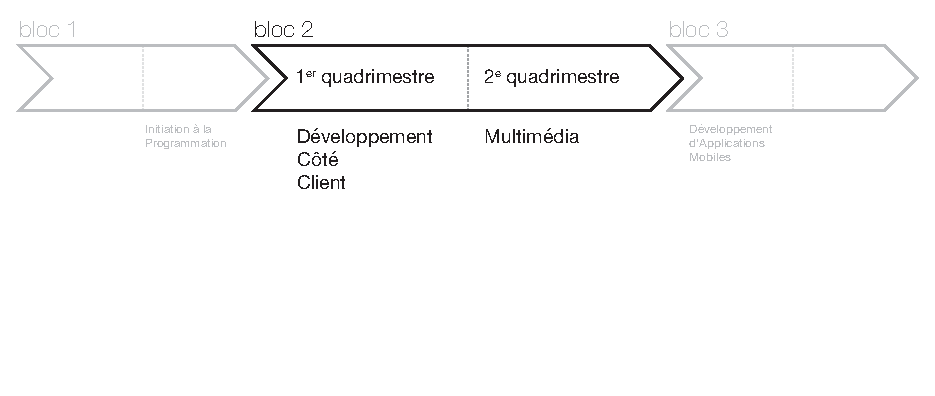
\includegraphics[width=\textwidth]{figures/corequis.eps}
        \caption{Illustration des corequis}
        \label{Fig:GQM}
    \end{center}
\end{figure}
\clearpage

\section{Contenus}

Voici dans l'ordre les différents thèmes que nous aborderons ensemble en classe :
\begin{enumerate}
    \item Réalisation d'un test formatif pour mesurer votre niveau en JavaScript.
    \item Rappel des concepts de base JavaScript utilisés dans le cadre de ce cours.
    \item Utilisation d’un framework pour compiler les fichiers sources.
    \item Réalisation d'animations 2D simples avec JavaScript.
    \item Réalisation d’un outil qui permet de générer un logo à partir de paramètres encodé par l’utilisateur.
    \item Introduction à l’API de Canvas.
    \item Révision de quelques concepts mathématiques essentiels pour animer des formes. (Radian, degré, périmètres, Sin, Cos, etc.).
    \item Mise en place d’une boucle d’animation. Déplacer aléatoirement et à vitesse constante, des formes dans un canvas.
    \item Déplacer plusieurs formes avec la détection du survol de la souris.
    \item Détecter et interagir avec les évènements émis par l'utilisateur. Clic, survol, clavier, etc..
    \item Utilisez l’API Canvas pour appliquer des traitements sur des images bitmap.
    \item Déplacer des formes avec des images dans un canvas.
    \item Aborder quelques éléments de physique élémentaire. Faire tomber de la neige..
    \item Dessiner et animer le décor d’un jeu 2D avec une sprite sheet.
    \item Réalisation d’un premier jeu complet Flappybird.
    \item Réalisation d’un deuxième jeu complet Asteroids.
    \item Réalisation d’un examen formatif des années précédentes.
    \item Correction de l'examen formatif.
\end{enumerate}

\clearpage
\section{Visées d’apprentissage}
\begin{itemize}
    \item Savoir programmer des interfaces multimédias riches dans un navigateur.
\end{itemize}

Nous nous limiterons, dans ce cours, aux jeux interactifs à 2 dimensions\footnote{Les jeus interactifs à 2 dimennsions sont par essence des interfaces multimédia riches.} en utilisant de manière conjointe l’API de dessin canvas et les bases du langage JavaScript.

\section{Méthodes d’enseignement et activités d’apprentissage}

Vous avez choisi un bachelier professionnalisant, qui cherche donc à vous préparer, au mieux, au mode professionnel. C’est  pourquoi j’ai choisi d’articuler l’acquisition des nouveaux savoirs autour de cas réels du jeu vidéo. Le cours se donne au deuxième quadrimestre, une fois par semaine à raison de 4 heures.
\begin{enumerate}
    \item Développer des solutions algorithmiques, dans une forme d’autonomie individuelle ou collective, avec vos connaissances ou en allant chercher d’autres, sur base d’un problème authentique issue du monde du jeu vidéo. Par exemple, comment détecter la collision de 2 formes dans un plan à 2 dimensions ? Ces solutions algorithmiques évolueront jusqu'à devenir des jeux complets.
    \item Je vous présenterai régulièrement les éclairages théoriques nécessaires à la compréhension de ces concepts algorithmiques. Parfois "après l’exercice" dans quel cas l’activité s’apparente plutôt à de l’exploration. Et d’autres fois "avant l’exercice" dans quel cas l’activité s’apparente plutôt à de l’exercisation et de manière plus générale à un apprentissage par problèmes. Au fil des semaines, vous travaillerez de plus en plus en autonomies étant donné que la matière vue augmentera.
    \item Je vous proposerai des petits exercices récapitulatifs qui abordent la manière déjà vue. Ces exercices couvrent de manière progressive la matière du cours. Ces derniers sont à réaliser en pleine autonomie chez vous. Certains exercices feront l'objet d'une correction collective en classe. Dans tous les cas, toutes les solutions sont disponibles.
    \item En tâche de fond, durant les différentes semaines de cours, vous devez réaliser, individuellement, un jeu que vous aurez choisi parmi le \href{https://fr.wikipedia.org/wiki/Liste_de_jeux_Atari_2600}{catalogue Atari}\footnote{Ce catalogue comporte 2600 jeux}. Il s’agit là d’une occasion de vous entrainer à l’examen et de revoir les points de matière du cours. Je vous encourage, au fur et à mesure que nous voyons les concepts théoriques, de les mettre en pratique dans votre jeu. (Voir section \ref{eval_formative} sur l'évaluation formative.)
\end{enumerate}

\clearpage
\subsection{Justifications}
\begin{itemize}
    \item Étant donné que la motivation fait partie de ma philosophie et que l’un des ingrédients de la motivation c’est d’apporter du sens aux connaissances, l’approche intégrée me permet de rendre concrets mes enseignements au travers de besoins issus de situations authentiques. Concrètement, j'articule la matière autour de besoins afin de faire ressentir l'intérêt de ces connaissances. Régulièrement, quand la plupart des étudiants ont trouvé une solution, je désigne quelques étudiants pour qu’ils présentent leur solution de sorte à introduire dans un troisième temps la théorique (Activité 1.2). J’ambitionne ainsi de susciter leur intérêt pour la matière puisqu’ils partent de situations plutôt complexes et authentiques. Il s’agit là des deux évènements dominants d’une séance de cours type.
    \item L'apprentissage par problème que je met en place, quand les étudiants doivent trouver la solition vise à développer leur autonomie sans pour autant les submerger, avec un problème trop compliqué. Dans l’activité 1.1, le problème reste simple. En revanche pour l'activité "projet" l’autonomie est encore plus forte. Avec un problème plus authentique et compliqié. Nous basculons vers un apprentissage par projet.
    \item "Make learning visible"\footnote{The ‘visible’ aspect also refers to making teaching visible to the student, such that they learn to become their own teachers.}\cite{hattie2012visible}. Le projet est une occasion pour l'étudiant de se rendre compte des savoirs qu'il acquière. Il voit bien qu'au fur et à mesure que la matière est vue il peut aussi avancer dans la réalisation de son jeu.
    \item \cite{perrenoud1992differenciation} dit "différencier, c’est organiser les interactions et les activités de sorte que chaque élève soit constamment ou du moins très souvent confronté aux situations didactiques les plus fécondes pour lui". Autrement dit, face à la diversité mathétique, il faut apporter une polyvalence didactique. J’ambitionne au travers de ces différentes méthodes de répondre à la diversité mathétique. C’est pourquoi à certains moments je laisse les étudiants explorer la documentation officielle de sorte à expérimenter les éléments dont ils ont besoin. Et d’autres fois, je leur donne d’abord les éléments dont ils ont besoin et puis ils appliquent la connaissance.
    \item Le projet donne aussi un sentiment de controle...Le fait que les étudiants sont libre d'organser leur temps pour le projet leur donne un sentiment de controlabilité. Voir (Rolland Viau)
    \item Etaillage... les cours doivent etre correctement calibrés. La complexité augmente pour donner le sentiment de compétences....sans jamais etre trop facile....

\end{itemize}
\clearpage

\section{Évaluation des apprentissages}
\subsection{L’évaluation formative}
\label{eval_formative}
\begin{enumerate}
    \item À la deuxième séance : vous réaliserez un test formatif d’application pratique du cours de "Développement côté client" qui est le corequis de ce cours. Ceci est occasion pour vous et moi de mesurer votre maitrise en JavaScript.
    \item À l'avant-dernière séance de cours : vous réaliserez individuelle un examen des années précédentes en classe. Nous consacrerons la dernière séance à sa correction collective où chacun corrige individuellement sa copie d'examen.
\end{enumerate}

\subsection{L’évaluation certificative}

L’évaluation certificative s'organise en 2 temps :
\begin{enumerate}
    \item Vous devez rendre, le jour de l'examen, via GitHub, votre projet de jeu personnel que vous aurez développé individuellement chez vous pendant les différentes semaines de cours. Les consignes vous seront communiquées au premier cours. Vous devez donc gérer ce projet qui compte pour 20\% de la cote finale.
    \item L'examen pratique, qui aura lieu le jour de l'examen. Vous devrez programmer un jeu à partir d'un énoncé\footnote{Je vous rappelle que les énoncés des années précédentes sont disponibles sur l'\href{https://github.com/tecg-mmi}{organisation GitHub} officielle du cours.} qui vous sera fourni et que vous découvrirez le jour même. Vous aurez à votre disposition toutes les ressources du cours, un accès aux documentations officielles, ainsi que vos propres productions. Vous disposez de 4 heures pour réaliser cet examen en classe. Ce travail compte pour 80\% de la cote finale. Vous serez dans une situation nouvelle, je ne reprends pas d'anciens examens puisqu'ils sont publics.
\end{enumerate}


\subsection{Justifications}
\label{evaluation_des_apprentissages_justifications}
\begin{itemize}
    \item "L’émission de feedbacks est souvent considérée comme un élément clé pour renforcer la motivation et soutenir la réussite des élèves."\cite{georges2011feedbacks}. La réalisation de l'examen formatif ainsi que le projet personnel (activités 2.1 et 2.2) sont 2 activités intégrées qui permettent à l’étudiant de recevoir du feedback. D'une part, sur sa compréhension de la matière, donc plutôt un feedback simple de type assertif et évaluatif \cite{georges2011feedbacks} sur sa performance. D'autre part un feedback plus complexe relatif aux stratégies qu'il faut adaptées. Par exemple, quelles sont les parties plutôt simples et comment rapidement les valider. Ou encore, réfléchir aux éléments plus compliqués, que mes étudiants aiment appeler des "pièges"\footnote{Je n'adhère évidemment pas à cette appellation. Mon examen ne contient pas de "pièges" sans quoi on pourrait se poser des questions sur mes intentions. L'examen contient des parties plus compliquées qui nécessitent une certaine forme d'inhibition cognitive.}. \citep{hattie2008visible} explique dans son ouvrage que le feedback a un impact significatif sur la performance de l'étudiant. Enfin, c'est une occasion pour entrainer la méta-cognission\cite{leclercq2008modele}. Nous réfléchissons ensemble aux stratégies qu'il faut mettre en place pour réussir l'examen. D'ailleurs chaque année je désigne un "sécrétaire" pour ces séances. Il aura pour mission de prendre note de toutes les astuces que nous avons déterminées ensemble afin que les étudiants puissent consulter cette ressource plus tard.\todo{Changer de place ?}
    \item La réalisation de l'exercice formatif est l'occasion pour moi de me rendre compte des éventuelles lacunes de certains étudiants. Cela me donne un vision assez précise du niveau de mes étudiants. Je peux donc donner un feedback personalisé à certains étudiants et surtout l'occcasion de leur fournir des ressources spécifiques.
    \item Parler de la correction des exercices....
    \item Hattie : To make learning visible... montrer que les étudiant ont acquis des chose. Ils ne sont pas venu pour rien...Il faut donner aux étudiant l'occasion de revenir sur les mêmes choses...
\end{itemize}

\section{Triple concordance ou alignement pédagogique}
\begin{table}[H]
    \begin{tabular}{|l|l|}
        \hline
        Visées d’apprentissage        & \begin{tabular}[c]{@{}l@{}}Savoir programmer des interfaces multimédias \\ riches dans un navigateur.\end{tabular}                                                                                                                                                                                                        \\ \hline
        Activités d’apprentissage     & \begin{tabular}[c]{@{}l@{}}- Exercice pratique par matière\\ - Entrainement à l’examen\\ - Exploitation collective ou individuelle de nouvelles \\  techniques pour proposer des solutions. (Apprentissage par problèmes)\\ - Apprentissage par projet avec le projet personnel.\\ - Transmission théorique.\end{tabular} \\ \hline
        Évaluation des apprentissages & \begin{tabular}[c]{@{}l@{}}Réalisation en classe d'un jeu en 2 dimensions\\ dans un navigateur avec l'API de canvas.\end{tabular}                                                                                                                                                                                         \\ \hline
    \end{tabular}
\end{table}

\subsection{Justifications}

\section{Modalités organisationnelles}
\subsection{Comment me contacter}
\begin{enumerate}
    \item Pour toutes les communications d'ordre personnel, je vous demande de me contacter par mail \href{mailto:daniel.schreurs@hepl.be}{daniel.schreurs@hepl.be}
    \item Si vous avez des questions techniques liées à une incompréhension et/ou un problème avec un exercice, je vous demanderai de la poser sur le Forum officiel du cours sur Moodle. Cela permettra de faire profiter tout le monde de votre question.
    \item Si vous avez des informations urgentes à me faire parvenir, vous pouvez me joindre directement via Teams que j'ai installé sur mon téléphone.
\end{enumerate}


\clearpage
\printbibliography

\end{document}
